%===================================== CHAP 4 =================================

\chapter{Experiment}

\section{Overview}
\label{sec:experiment_overview}
As presented in Section \ref{sec:problem_statement}, we wanted to do test an architecture that allows fully decentralized machine learning that maintains the privacy of the participants. 

We consider a setting with $N$ peers that each have a local data set. These data sets are assumed to be independently sampled for each peer, but may be sampled from the same distribution. When the system initializes, each peer trains a logistic regression model on its local dataset. The data set and the trained model is private and should only be known by its owner.

After the initialization phase, the aggregation phase begins. In this phase, the aggregation mechanism described in Section \ref{sec:Sensitivity_of_LogReg} is applied one or more times, using the private model held by each peer. The mechanism is not applied to all peers at the same time. Instead, subsets of peers are selected randomly to form aggregation groups, each group producing a single aggregate model. Many such groups can be formed, and the group size can vary from including all the available peers to including just a single peer. In our experiments, we specify a constant group size which is used until the end of the experiment.

While the output of each mechanism application is an average of the input models, produced in way that guarantees differential privacy, the computation itself must be done in a central manner. This is possible to do securely using the protocol detailed by Pathak et al., which uses homomorphic encryption to compute the model aggregate without allowing the any of the participants to know the original, private model of another participant\cite{pathak2010diffprivhomo}. Since this protocol requires some central computation, one of the peers is chosen at random to be the curator, responsible for acting as the central party described in the solution by Pathak et al. The other peers in the group will submit the necessary information to this curator, including their private model, in an encrypted fashion. Once the peer acting as curator has received a model from all participants, it computes the average model, adds noise sufficient to guarantee $\epsilon$-differential privacy and publishes the final result. The target of this publish step can vary. In our experiments we have tested one version that publishes a model to all available peers and one that only publishes the model to the peers in the group that helped create it.

Each peer holds a privacy budget, as discussed in Section \ref{section:privacy_budget}, that limits how many times it can be involved in a mechanism application. If the budget of a peer is depleted, it is no longer a candidate for the randomly formed aggregation groups. When there no longer is enough peers to form a group with the size specified for a particular experiment, the experiment terminates.

\subsection{Limitations of current implementation}

Certain parts of this system is not implemented in this project, and are replaced by black-box substitutes that simulate the required behavior. We have only done this for components that are already described and tested in other work. 

The protocol created by Pathak et al. for computing aggregates securely was not implemented. In our implementation models are sent unencrypted to the peer acting as curator. While this part would need to be replaced with a full implementation of the approach by Pathak et al. the output returned by the curator is exactly the same, using the computation in Equation \ref{eq:parametric_aggregation}. 

Finally, the selection of random groups is done in a non-scalable manner. A centralized actor that has full knowledge of all participating peers randomly selects groups of these peers and sends a message to each peer with the list of participants. This should be replaced by a decentralized method for the system to be scalable. How we intend to do this is discussed further in Section \ref{sec:Future Work} on Future Work.

\todo[inline]{Make an explicit assumption that Pathaks protocol is secure and can compute the result as we described in basic theory. Explicit assumptions are important.}

\section{Architecture}

We designed a distributed system using the JADE framework. The core component in this system is a PeerAgent, which represents a participant in the distributed learning setting. This agent contains what would be the local data of a person using some application. In the remaining sections, whenever we say "peer" we are refering to the PeerAgent described here, holding a local data set and with means of communcating with other PeerAgent instances.

To form aggregate models it is necessary to select groups of peers to create each model. In our experiment, this is implemented with a singleton agent we named the GroupAgent. This agent draws random subset of size $g$ from the set of all peers. The size and number of groups formed is given by parameters selected at the beginning of the experiment, which are described in detail in Section \ref{sec:parameter_tuning}. 

As stated in Section \ref{sec:experiment_overview},  the experiment terminates when there no longer a sufficient amount of active peers to form a group. That is, when the number of peers with sufficient budget is less than the group size parameter, the experiment is stopped. This behavior was implemented into an agent we named CompletionAgent. This agent listens to messages from the curators in the different groups. Once it has received messages of the expected number of aggregated models having been created, it initiates the final step of the experiment, including testing performance metrics and preparing the JADE environment for the next experiment. 
%talk about how the stuff explained in Basic theory like AMS plays into our setup

%when we are talking about peers, we are refering to instance of the PeerAgent


\subsection{Communication}
\subsubsection{Peer}
\todo{Model training on agent instantiation.}
How is each peer set up, and what behaviors do they implement? 
How do they update then propagate the model being learned.
How do they know when to stop?
\subsubsection{messaging}
How do the peers communicate with each other?
What does a message look like?
What is the PeerGraph?
What controls the messages and determines where they should go?
\begin{figure}[h!]
	\centering
	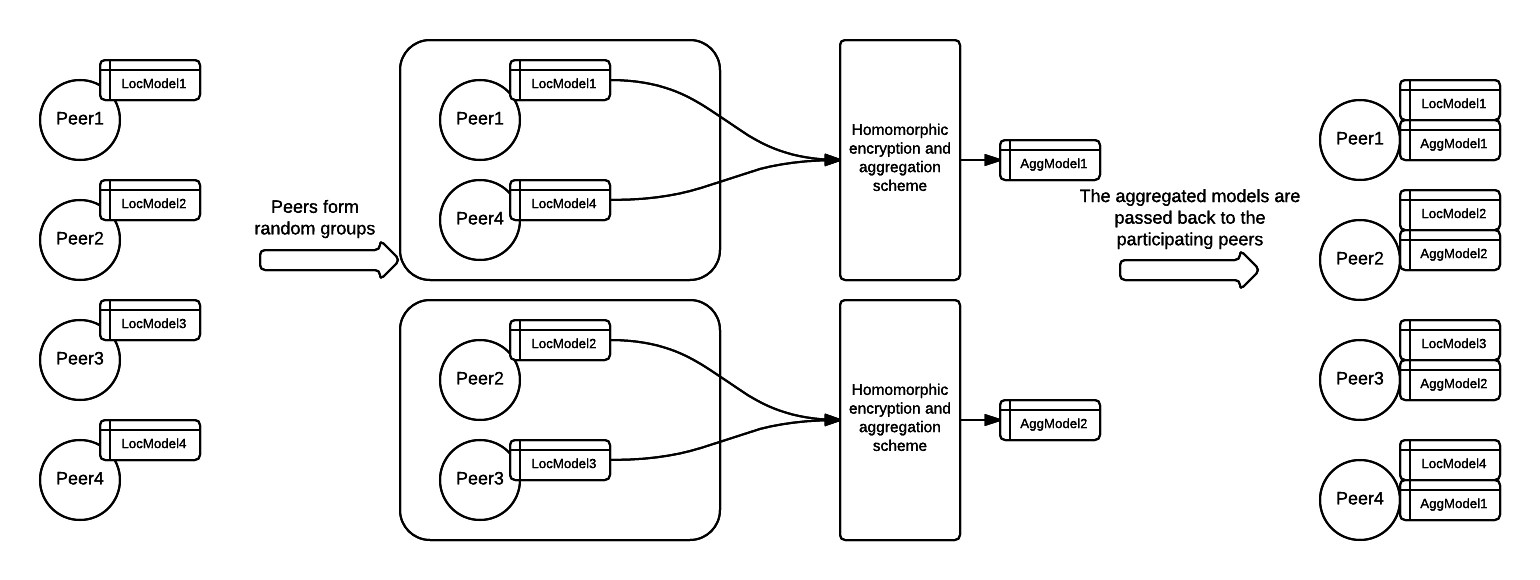
\includegraphics[width=\textwidth]{fig/peerModelCreation}
	\caption{One iteration of model aggregation}
	\label{fig:peerAggregationFigure}
\end{figure}

\section{Dataset and preprocessing steps}
\label{sec:datasets}
This section will introduce the dataset(s) used. What features it contains, what we try to learn/classify, and why we chose to use it.

Each data set was divided into a training set partitioned among the peers in the system, and a testing set not used until the very end of our project, to verify the results indicated in cross validated experimentation. How the test set was selected is specified later for each data set.
A feature with constant value 1.0 was appended to all data records before fitting models, to act as the intercept or bias term. When necessary we scaled the features of the data sets to 0-1 range. This is due to the proof in Chaudhuri paper which states the assumption $|X_i|\leq 1$. The scaling was done by the formula

\begin{eqnarray}
X_{norm} = \frac{X-X_{min}}{X_{max} - X_{min}}
\end{eqnarray}

$X_{min} and X_{max}$ were calculated using only the training set of each data set, to avoid leaking information about the test set into the training set. The test sets were then scaled in the same manner using the same $X_{min}$ and $X_{max}$ as calculated on the training set.

This is a potential source of unrealistic information leakage. In a real implementation, globally determining scaling on the training set would be difficult. Instead, it might be necessary to perform this scaling locally at each peer. This means that the scaling constants $X_{min}$ and $X_{max}$ would be at least somewhat different for each peer, and would only be calculated on their particular partition of the training set. We performed the scaling globally on the training set because we believe any effect from this to be small. In particular, it does not detract from the conclusions we make that are the most relevant to our research question, which relates to usefulness of model aggregation and any options we identify to reduce standard deviation across the peer population.  \todo[inline]{Give a compelling reason for why this is. OR - consider making scaling a local problem. This could actual improve our results as it pertains to aggregation usefulness.}

\subsection{Spambase} \label{sec:spambase}
The Spambase dataset \cite{spambase1999data} was used as a baseline training set. This dataset is publicly available from the UCI machine learning directory, and contains 57 input attributes of continuous format which serves as input features for spam detection and 1 target attribute in discrete format which represents the class.

We chose this dataset as it is a popular dataset to analyze the performance of binary classifiers, so that we could compare the results of other logistic regression classifiers against our own. While this dataset might not seem like the ideal choice for testing a differentially private classifier due to its lack of personal information, we argue that it still fits well for the purpose of demonstration. In a spam-classifying system based on our distributed model, a logistic regression model can be built by training it locally in each user's personal mail folder and then aggregated into an ensemble. That way you can build a diverse spam-classifier without the users having to give up their personal email to a centralized database.     

We randomly partitioned this data set into a training set and a test set, with 80\% of the records in the training set and the remaining 20\% in the test set.

\subsection{Australian Credit Approval}
Another dataset we used, was the Australian Credit Approval (Statlog), which concerns the approval or disapproval of credit card applications. It is publicly available from the UCI machine learning directory. This is a much smaller set of data, with only 690 samples spread over 14 attributes. The data is useful for binary classification as it contains a good mix of attributes: continuous, nominal with small numbers of values, and nominal with larger numbers of values.

We mostly used this dataset to confirm and double-check the conclusions we drew from the Spambase dataset, as it contains too few data records for it to be 100\% ideal for our use. Due to the sparsity of data we had to scale down the amount of peers in each experiment, so that each peer could get enough data to create a decent local classifier. We chose to keep on using this data as one of the motivating examples in Dwork's book\citep{dwork2013algorithmic} on the applications differential privacy, is to protect data holders from insurance and credit card companies. 


\subsection{Adult}
As we needed a larger dataset to enable us to scale the amounts of peers in the experiments, we chose to use the Adult dataset from the UCI machine learning repository.  It consists of personal information records extracted from the US census database and the task is to predict whether a given person has an annual income over or under \$50,000. The original Adult data set has six continuous and eight categorical features. We
downloaded the dataset pre-processed by \cite{platt1999fast}, where the continuous features are discretized into quintiles, and each quintile is represented by a binary feature. Each categorical feature is converted to as many binary features as its cardinality. The dataset contains 32,561 training and 16,281 test instances each with 14 features.

This dataset is very popular to use in various machine learning experiments, ranking second on the download list for the UCI machine learning repository. This dataset has also been used before in research in privacy research, most notably in the work by \cite{pathak2010diffprivhomo}. This has given us some baselines to compare our own results against \todo{Put in a ref to baseline table}].

\section{Parameter tuning}
\label{sec:parameter_tuning}
Number of peers $P$ specifies how many different peers participate in the experiment, and necessarily the number of partitions of the training data sets. The training is divided into $P$ parts of equal size.

\todo[inline]{Rationalize why we have included 1 in the 10-inteval experiments - it is because 1 is a very interesting edge case. Should also talk about the significance of group size 1  in analysis.}

Aggregate models are created from local models at each peer through an aggregation process that is performed one or more times with subsets of peers. The parameter $g$ specifies how many peers will participate in a single model aggregation. Since each peer has a unique subset of data, this parameter determines how many partitions of the training set contribute to the published aggregate models. These data partitions do not contribute directly, but indirectly through the aggregation of models trained locally on each partition.

The privacy parameter $\epsilon$ determines the level of privacy required for each peer and its set of data instances. Note that this parameter does not apply to the original training set as a whole - each peer has its own private database, which is protected by $\epsilon$-differential privacy. 

Each peer will get $R$ number of records. This parameter will obviously have a significant effect on how well the local model each peer creates is able to generalize to new data instances. 

Each peer trains a local logistic regression classifier on its data partition. This requires selection of an adaptive learning rate parameter $\eta$, a regularization constant $\lambda$ and a maximum number of epochs of stochastic gradient descent. We tuned $\eta$ by running 3-fold cross validation when each peer fits its local model to identify the best $\eta$ by powers of 10 in the range $[10^{-2}, 10^{2}]$. When using SGD with adaptive learning rate, this range proved sufficient to find classifiers that were as good as our best baseline throughout experimentation. 3-fold cross validation was chosen because of both project computer time constraints and experimental data constraints. Each experiment in its entirety is tested with 10-fold cross validation, so it was necessary to reduce local model training time in order to run in a reasonably short time on a single computer. The data constraints is a part of the domain we want to explore. When the amount of data is very small, 3-fold cross validation offers a balance between parameter search reliability and validation set sizes.

In usual data mining applications the regularization $\lambda$ would be tuned in this manner as well, but the sensitivity of the aggregation mechanism depends on $\lambda$, as seen in Equation \ref{eq:aggregated_logistic_sensitivity}. This means that the peers will have to communicate to either agree on a regularization level or to determine the smallest regularization constant to identify the worst case noise level. In our experiments we chose a global regularization level, which was used by all peers. We identified the best $\lambda$ by testing a coarse grid of powers of 2 in the range $[2^{-8}, 2^{8}]$ whenever we tested with a new data set. If several values of $\lambda$ presented similar prediction performance results, we chose the highest value. This is both motivated by a desire to have each model generalize as well as possible to future data instances and the fact that lower values of regularization increases the noise added in model aggregation.

When we wanted to test a new number of records per peer $R$ or the privacy level $\epsilon$, we re-tuned $\lambda$ to ensure that it had the optimal value. This is necessary, since a lower number of records can mean that higher regularization is necessary. Additionally, a lower value of $\epsilon$ increases the variance of noise added to the aggregated models. This effect can be mitigated by increasing regularization. \todo[inline]{We should also discuss possible problems with this approach.} The manner in which we choose $\lambda$ should be considered a bit of an optimistic approach. In reality, global cross validation to determine best regularization is not practical and would create challenges with the privacy guarantees. Since we mostly experimented with less than 100 peers, we believe our global cross validation is reasonable close to an approach were peers cooperate to pick the strongest possible $\lambda$ with acceptable performance on average.

Finally, the parameter $\epsilon$ can be divided across several applications of the aggregation mechanism, as described in Section \ref{section:privacy_budget}. This was achieved with a per-aggregation parameter $\epsilon_i$. Each data partition can participate the aggregation mechanism $n$ times, where $n\epsilon_A \leq \epsilon$.

\section{Validation}

The test sets set created as described in Section \ref{sec:datasets}. These test sets set aside could not be used when tuning and evaluating our solution. In order to explore the effects of the various parameters we used cross validation with number of folds $n=10$. For a given combination of parameters, performance metrics were measured as their average across ten repetitions. In repetition $i$, data fold $i$ was used as validation set and the remaining $n-1$ data folds were combined to form the test set.

Following the approach outlined in Section \ref{sec:parameter_tuning}, we established suitable ranges of logistic regression hyperparameters, before proceeding to testing with different levels of privacy, peer numbers, group sizes and record numbers. Once we felt confident that we had established a set of experiments that as far as possible could answer our research questions, we performed. All numbers reported in Chapter \ref{chap:analysis} are average measures on the test set across ten full executions of the experiment, with the training set being randomized before each iteration.

\todo[inline]{Explain the risks of not having used stratified CV, especially with Adult}

\todo[inline]{Justify the usage of Mean classification error. Why is it okay that we focused less on TP and FP rate, and so on.}

\todo[inline]{Explain how we are measuring standard deviation - and explain that there are two notions of variance that we test - across iterations and peer }

\section{Experiment execution}

For each experiment, we selected a single parameter of the set of parameters specified in Section \ref{sec:parameter_tuning}, for which we wanted to explore the behavior of the system as the parameter took a range of values. specified a range of values for the parameter we were experimenting with. fixed, scalar values for each of the parameters described in Section . For example, one of the experiments we performed was intended to test the effect of varying number of peers participating in the system. One possible parameter combination to test this could then be

$$P=[10, 20, 30, 40, 50], G=10, \epsilon=0.1, \epsilon_{A}=0.1, \lambda=1.0$$

Then a full simulation with $p$ peers is repeated and evaluated 10 times, either by cross validation or test set, for each $p$ in the specified parameter set $P$. 

\subsection{The execution of a single experiment}

As previously stated, each set of parameters was tested 10 times - across 10 folds for when we validated with cross validation and over 10 repetitions when we tested against the test set.

For each of these iterations, there is a set of instances used to train logistic regression models, and a set of instances used to quantify the predictive performance of the peers after the number of aggregations available given a particular combination of $P$, $g$, $\epsilon$ and $\epsilon_A$ have occured. In the following sections we give in more detail the steps we used to perform our experiments given this set of training and testing instances.

\subsubsection{Instantiation}


First, the data is shuffled. This is done since the exact way in which the data is distributed among the peers can have a significant effect on the quality of their. If each peer was given thousands of records these partitions would likely be fairly uniform, and shuffling the training data would be less important. However, since we wanted to experiment with data quantities below 100 instances per peer, we expected significant variance in the trained models. The data is partitioned into $P$ partitions, with equal size. $P$ instances of PeerAgent is created, and the one partition of training instances are given to each peer.

\subsubsection{Fitting Local Classifiers}

Once the environment is set up, all agents are registered and the peers have been given their data partition, the peers fit a logistic regression model to the data they have been given. The model fitting is done by mini-batch SGD as described in Section \ref{sec:gradient_descent}. Each peer runs 3-fold cross validation over a single epoch to determine the optimal $\eta$, and picks the $\eta$ which has the lowest average prediction error on average. When $\eta$ has been determined, the logistic regression model is fitted to the peers local data, with the chosen $\eta$ and the $\lambda$ specified for that particular experiment. The fitting is done by running mini-batch SGD for a maximum of 100 epochs.

\subsubsection{Application of Aggregation Mechanism}

After all peers have fitted their local classifiers, the aggregation phase begins. The GroupAgent has a list of the peers that still permit their locally trained classifiers to take part in a published, perturbed model. While there still is enough peers to form a set of size $g$, the GroupAgent randomly selects a subset of these peers. Among this subset, it randomly picks one peer to act as the curator, responsible for performing the steps that result in an aggregated model that can be published with a differential privacy guarantee. It then sends a message to each of the selected peers.

Once a PeerAgent is notified that has been selected to be the curator of a group, it starts waiting for messages from the other peers in the set. The other $g-1$ peers that are selected to be contributors will send their local classifiers to the curator as soon as they are notified by the GroupAgent. When the peer acting as curator has received all the $g-1$ models, it applies the aggregation mechanism given in Algorithm \ref{alg:privacy_mechanism}. It includes its own local classifier in this step, which produces a final aggregate model from $g$ other models. 

As presented in Section \ref{sec:Sensitivity_of_LogReg}, the sensitivity of logistic regression depends on the sizes of the data sets used to train the models. Specifically, the mechanism needs to know the size of the smallest training set in order to guarantee differential privacy. It is important to note that the method we are testing assumes honest-but-curious participants, as assumed by \cite{pathak2010diffprivhomo}.

\todo[inline]{Make it a bit more explicit that this is Pathaks mechanism, essentially, without the Homomorphic encryption.}

\begin{algorithm}[!h]
	\label{alg:privacy_mechanism}
		\KwIn{$\epsilon$ - privacy parameter
			$\boldmath{M}$ - set of models trained by participating peers\;
			$\boldmath{N}$ - set of peer training set sizes\;
			$\lambda$ - regularization level used when training each model in $\boldmath{M}$\;
			}
		\KwOut{Perturbed aggregate of the models in $\boldmath{M}$}
		$n_{min} \leftarrow min(\boldmath{N})$\;
		$\eta \leftarrow Laplace(0; \frac{2}{n_{min}\epsilon\lambda})$\;
		$model_{agg} \leftarrow 1/K\sum_{j=1}^{|\boldmath{N}|} \boldmath{w_j} + \boldmath{\eta}$\;
		\KwRet{$model_{agg}$}
		
\caption{$\epsilon$-differentially private aggregation mechanism}
\end{algorithm}


\begin{algorithm}[!h]
	\KwIn{$P$ - the set of peers\;
		$\epsilon$ - privacy parameter\; 
		$\epsilon_A$ - privacy level of a mechanism application\;
		$A$ - the $\epsilon_A$-differentially private aggregation mechanism\;
		$group\_size$ - number of peers in a single mechanism application}
	\For{peer $\in$ P}{
		$budget_{peer} \leftarrow \epsilon$\;
	}
	\While{$|P| \geq group\_size$}{
		$group \leftarrow randomSample(P, group\_size)$\;
		$model_{agg} \leftarrow A(group)$\;
		\For{peer $\in$ group}{
			$budget_{peer} \leftarrow budget_{peer} - \epsilon_A$\;
			\If{$budget_{peer} < \epsilon_A$}{
				$P \leftarrow P \smallsetminus peer$\;
			}
		}
		$publish(P, model_{agg})$
}
\caption{Application of aggregation mechanism}
\end{algorithm}

\todo[inline]{Defend randomSample procedure using Newscast reference}



\subsubsection{Propagation Of Published Models} \label{sec:PropagationPubModel}

Originally in our system, aggregated models were only propagated to the peers that had participated in creating that model, as can be seen in Figure \ref{fig:peerAggregationFigure}. What resulted from this, especially when epsilon was set to a low amount such as 0.1 or lower, was that the high amount of noise made the classifiers have a big standard deviation on their mean classification rate. What this meant was that while the classifiers could be very accurate in some peers, classifying up towards 90\% accuracy, it could also be significantly worse in other peers. 

We theorized that we could improve the ensemble classifier in each peer if we could propagate the aggregated models to all the peers in the network, instead of just those who had participated in making them. Our hypotheses was that this would lead to more stable classifiers with lower standard deviation, due to a smoothing effect in having more models in the ensemble classifier in each peer. This is basically the same idea as bootstrap aggregating, or bagging, which has been proven to lead to improvements in unstable procedures\citep{breiman1996bagging}. 
\todo{Definitely talk more about the bagging effect, either here or in the analysis section}

For this reason, we decided to run experiments to compare the different possible model. In all cases, the published models will have been perturbed with Laplacian noise to give $\epsilon$-differential privacy. In the group publication setting, only the peers that join together to produce a perturbed model will receive the final result. In the full publication setting, all peers active in the network will receive all perturbed models. 

Note that there is no selection or pruning of the ensemble classifier owned by each peer. If a peer receives a model, it will blindly add it to the ensemble. This means each peers ensemble model will grow much faster in the full publishing setting, and they will all contain essentially the same models, the only exception being the unperturbed model produced by the peer locally. We anticipated that this would lead to a reduction in ensemble model accuracy variance.


\subsection{Reset of the experimental environment}

Between each execution of the experiment the JADE environment must be prepared for the next experiment. In our initial implementation we had problems with dynamically restarting the environment, as it was slow. For this reason, the experiment environment is reset by simply removing all PeerAgent instances and the GroupAgent. We still had problems with removing the CompletionAgent quickly enough to allow the experiments to execute without pause, so instead of removing this agent, we simply reset its state and reconfigure it with the next experimental setup.

Once the CompletionAgent is reset and the other agents are removed, the environment is prepared for the next experiment. If all iterations of testing has completed for the particular combination of parameters, the experiment moves to the next set of parameters. If not, the same parameter combination is tested once more. 

\section{Distribution}`
Introduce notion of distributed machine learning. 

Why did we choose to perform distributed learning?

How does it fit with the notion of differential privacy?

Can we guarantee differential privacy while doing it distributed

Record-based differential privacy. Does it work?

\todo[inline]{This section should maybe go somewhere else, but where?}


\cleardoublepage